\chapter{Introduction}\label{chap:introduction}
In this thesis, we propose a methodology of cascading sequence labeling models to extract metadata from scientific publications. The following chapter offers a compact introduction to the problem domain (Section \ref{sec:problem_domain}), provides a short overview over the GEOcite project (Section~\ref{sec:geocite}), presents the problems encountered in the GEOcite metadata extraction process and questions we are trying to answer (Section~\ref{sec:research_questions}), and provides an outline for the rest of this thesis (Section~\ref{sec:structure}). 

\section{Metadata in Scientific Publications}\label{sec:problem_domain}
Metadata, or literally \enquote{data about data}, as a concept, has existed since ancient times and in our increasingly digital world, we continue to interact with metadata more frequently than ever before.\\
Historically, the primary focus of library metadata has been to enable access to analog collections. As such, library metadata encompasses indexes, abstracts, and bibliographic records that adhere to cataloging standards such as the Anglo-American Cataloguing Rules (AACR) and the Machine-Readable Cataloging (MARC) format.\\
Online databases, such as bibliographic utilities, online public access catalogs (OPACs), and for-profit databases like Scopus, made the results accessible to a wide range of users~\cite{schmidt1997libraries}.\\
Constant technological advancements in automated data processing, like metadata mining and web crawling, as well as a increasing number of elaborate standards and concepts like the Resource Description Framework (RDF) and the Semantic Web, suggest the automation of metadata procession is expected to increase further~\cite{gill2008introduction}.
\newpage

An ever-growing amount of academic publications and journals per year~\cite{fire2019over} can impede effective data discovery for researchers. Metadata of scholarly work, consisting of information about the title, authors, abstracts, research topics, and keywords, plays a vital role in indexing for search engines like Scopus or Google Scholar~\cite{ahmar2018lecturers}. This facilitates the effective exploration and discovery of scientific publications, enabling scientists to locate and access relevant work within their fields of interest. By leveraging comprehensive metadata, researchers can navigate the vast landscape of scholarly literature with greater efficiency and precision by filtering unrelated information in their search queries.\\
Furthermore, Metadata can help with long term tracking and preservation of scholarly work. While storing and conserving whole publications is only possible with specific open licenses, metadata of those aforementioned articles generally do not fall under copyright protection~\cite{cox2017metadata}. This allows the creations of large digital archives to permanently store data for tracking, preservation, and an open or commercial exchange, independent of the copyright holder.\\
Metadata also helps with tracking of citations in scientific work by establishing links between citing and cited publications, creating graph-like networks. Online databases like Crossref~\cite{bartell_crossref_nodate} and DataCite~\cite{noauthor_datacite_nodate} enable citation linking independent of an article's publisher. Author-level metrics like the h-index~\cite{hirsch2005index} quantify the impact of a researcher's work and provide a theoretical evaluation of his/her academic career.\\
In the context of this thesis, we are foremost interested in two categories of metadata in scientific publications
\begin{itemize}
    \item metadata about the publication itself. Information, which can by itself or combined identify a document, for example, authors, title, abstract, or the date. Since it resides often in the header section of an essay, we will simply refer to it as \enquote{header metadata}.
    \item metadata about the cited scholarly work within a publication. Using the same aforementioned principle, we will refer to it as \enquote{reference metadata}.
\end{itemize}
Naturally, the question arises of how we can actually gather this data automatically, given an arbitrary scholarly article.
An intuitive first approach could resolve around unique identifiers of a documents. Persistent identifier, such as the Digital Object Identifier (DOI), International Standard Serial/Book Number (ISSN/ISBN), or the Publisher Item Identifier (PII) can be extracted from a document using simple regular expressions.
\newpage

The regular expression
\begin{Verbatim}[fontsize=\small]
/^10.\d{4,9}/[-._;()/:A-Z0-9]+$/i
\end{Verbatim}
matches 99.3\% of all of Crossref's DOIs~\cite{Gilmartin_2015}. The resulting identifier can then be used to query metadata about the publication directly from the Crossref or DataCite API.\\
This trivial approach falls short in reality, as we can not always reliably extract an unique identifier. The DOI standard, for example, was established in the year 2000. A theoretical algorithm utilizing DOIs for metadata queries would not be able to gather data about a publication written before the year 2000.\\
Furthermore, we might extract multiple identifiers, since DOIs can also be attributed to referenced literature.

\section{GEOcite}\label{sec:geocite}
To fully understand the underlying problem, we want to briefly introduce the GEOcite project, which essentially deals with the question of how we can automatically extract metadata from a large corpus of scholarly work. We further want to show shortcomings of this approach and illustrate, how recent advancements in Machine Learning (ML) might help to bridge this gap.

\subsection*{The GEOcite Project}
GEOcite is a research project funded by the German Research Council (DFG), which aims to make an empirical contribution to the scientific discussion about the practice of interdisciplinary work using the example of geography by means of network-analytical and bibliometric analysis \cite{geocite}.\\
It is designed as the direct continuation of the DFG project \enquote{Die Säulen der Einheit und die Brücken im Fach}\cite{geocite_dfg}, which aims to identify and analyze the interdisciplinary structures within the German-speaking scientific community in the field of Geography. While the previous research work was limited on presently existing structures, the focus of the current phase lies on the temporal evolution of this research network.\\
To investigate these relations within the Geography research community, the GEOcite project intends to analyze the citation behaviour of all German-speaking post-war professors in the DACH region since 1949. Resulting insights may contribute towards exploration of the genesis of various subdisciplines within the field of Geography, or examine the temporal shifting role of female researchers in this specific academic circle.
Subsequently, the resulting, graph-like citation networks can be evaluated using network analytical methods \cite{aufenvenne2014saulen}.\\
As a first step to create a citation network, a comprehensive database of all Geography professors from Germany, Austria, and Switzerland, which were active between 1949 and the present day was created \cite{geoprof}. Within the context of this thesis, members of this collated group of professors are also referred as actors.\\
In the following sections, we will briefly describe the fundamental architecture of GEOcite and current data transformation processes as well as drawbacks and possible improvements, suggested in this thesis.

\begin{figure}
	\centering
	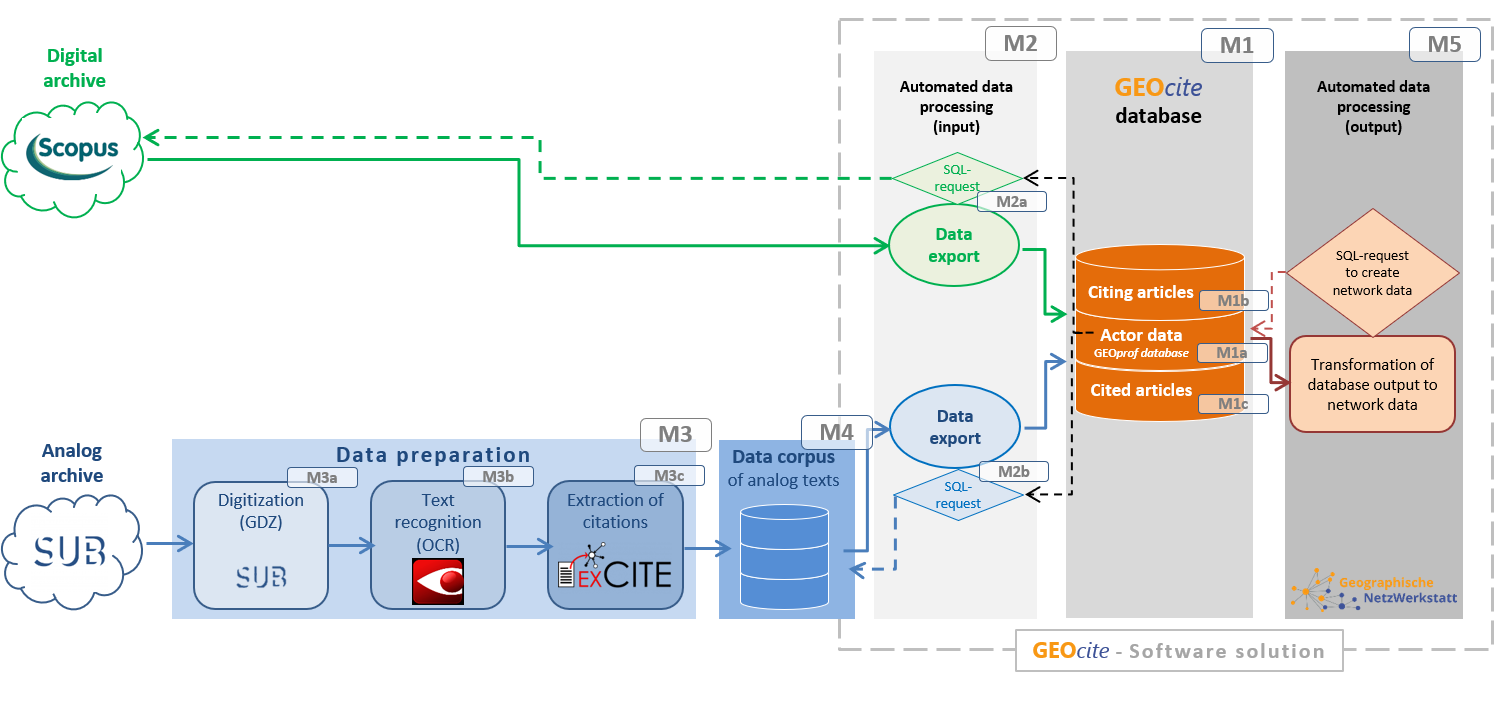
\includegraphics[width=1.0\linewidth]{images/geocite_dataflow_eng.png}
	\caption{The conceptional workflow of GEOcite.}
	\label{fig:geociteConcept}
\end{figure}

\subsection{Literature Sources}
The relevant literature is extracted from two distinguished data sources: from the citation database Scopus, in context of GEOcite referred as \enquote{digital archive}, as well as from a collection of analog scans of various journals, also referred as \enquote{analog archive}.\\
While Scopus is mainly used to gather metadata from recent publications of relevant actors and already provides parseable citation data via an API, the analog literature collection contains mostly articles from earlier years and requires several data processing steps to extract relevant information. Our analog corpus consists of 20,190 documents, predominately (85\%) in German. A large minority (14\%) consists of publications written in English. The remaining documents (1\%) are mainly of French and Spanish origin. In the scope of this thesis, we are primarily interested in the extraction process of citation data from the analog archive.

\subsubsection{Data Processing of Analog Data}
After the identification of relevant journals, articles are scanned and undergo several automatic pre-processing steps like conversion to grey scale images, skew correction, and noise removal. An OCR software is then applied to the processed scans, which are subsequently converted to PDF files with the corresponding text layer.\\
In the next processing step useful metadata about the article itself is extracted, for example author names, article title, journal, DOI, and date, which is needed to match an author of an article with an identified actor.\\
To extract this necessary header information about an scientific essay, the open-source software GROBID \cite{lopez2009grobid} is used. While it also possible to extract citation data with GROBID, GEOcite utilizes the EXCITE toolchain for this step~\cite{excite_toolchain}, specifically the EXParser component. Both EXParser and GROBID use a cascading composition of Machine Learning (ML) models to extract citation data. EXParser, however is specifically trained on German scholarly literature and is therefore more suited to our analog corpus. We will take a more detailed look on EXParser and GROBID in Chapter~\ref{chap:related}.

\section{Research Questions}\label{sec:research_questions}
The employment of two complementary tools to extract relevant information may cause friction under certain circumstances. Changes in IT infrastructure or updates can cause unforeseen compatibility issues. Modifications of existing processing routines can generate overhead work and prolong maintenance work. An unified tool, capable obtaining both header information, as well as citation data is therefore preferable.\\
Of all documents in our corpus, which are written in English, 91\% were published after the year 2000. This suggests that the trend to publish increasingly scholarly literature in English \cite{di2017publish} can also be observed in our corpus. GEOcite is designed as continuous project, with an ever expanding online and analog literature collection. Since EXParser is trained on scientific essays written mostly in German, we expect a declining performance on newly published literature, simultaneously historical documents become more accessible. To allow a future-proof data mining process, we require a ML model capable of extracting metadata from publications written either in German or English.\\
The processing pipeline of GEOcite involves the crucial step of transforming analog text into digital representations. To achieve this, OCR is employed to convert the physical documents into a machine-readable format. However, it is important to acknowledge that the OCR process is not infallible and can introduce errors or inaccuracies. Therefore, the aim is to construct a robust system that can effectively handle these imperfections.\\
Both GROBID and EXParser utilize Conditional Random Fields (CRF) as backbone for their information retrieval process, relying on textual and layout features. Visual information has proven to be valuable and effective when extracting data from visual-rich documents~\cite{cui2021document}. Continuous advances in Deep Learning, especially in the fields of Computer Vision, Natural Language Processing (NLP) and DocumentAI, suggest that these technologies can be used to improve the results of our extraction process.\\
We want to address these issues in this thesis, and want to offer a unified and robust solution for the metadata extraction process, utilizing state-of-the-art ML technologies and capable of working on multilingual literature. To explicitly summarize the aforementioned ideas, we want to answer the questions, if we can
\begin{itemize}
    \item simplify the structure of the extraction process and condense the functionally in one tool?
    \item employ a mostly language independent extraction process by utilizing multilingual ML models?
    \item create a robust system, that is able to handle impurities in our data?
    \item improve our overall extraction process by utilizing state-of-the-art ML technologies and techniques?
    \item include visual information to improve the results of our extraction process?
\end{itemize}

\section{Structure of the Thesis}\label{sec:structure}
In Chapter~\ref{chap:background}, we provide the background material for this thesis. Chapter~\ref{chap:related}, contains related approaches, available software solutions, and datasets related to our problem domain. Chapter~\ref{chap:methods} explains the methods, we used to answer our research questions. We provide a conceptual framework, explain our approach, and describe our data collection as well as the models employed. In Chapter~\ref{chap:bibex} we present our application, BiBEx, we developed to address the problems encountered in the GEOcite metadata extraction approach. The results of our overall system evaluation as well as the component evaluation of our system are presented in Chapter~\ref{chap:results}. We discuss our results and the limitations of our work in Chapter~\ref{chap:discussion} and conclude our thesis in Chapter~\ref{chap:conclusion} and highlighting potential future work.
